\chapter{The Architecture of Modern AI IDEs (Cursor, Claude Code, Canvas)}

AI coding platforms like Cursor, Claude Code, and ChatGPT Canvas differ from standard code generation APIs. They do not simply write code blocks on demand; they run continuous, background-driven coordination loops that monitor the workspace state, run AST indices, and apply edits directly to active file buffers.

\section{The AI IDE Execution Loop}

When you ask Claude Code to ``fix all linter warnings in this workspace,'' the client initiates a background execution loop:
\begin{enumerate}
    \item \textbf{Workspace Observation:} The agent scans modified buffers, diagnostics (warnings, errors), and active terminal states.
    \item \textbf{Action Selection:} The model chooses to read a file, run a bash command, or search for definitions via an LSP (Language Server Protocol) server.
    \item \textbf{Self-Correction Gate:} If the compilation fails, the compiler errors are fed back into the context window, allowing the agent to self-heal.
\end{enumerate}

\section{Line diffing: The Myers Diff Algorithm}

If an agent wants to edit a 5,000-line codebase file, sending the entire file back and forth is cost-prohibitive and slow. Instead, the model outputs a search-and-replace block, and the IDE computes a line diff to apply the changes.

The standard diff engine is powered by the \textbf{Myers Diff Algorithm}, which resolves the Shortest Edit Script (SES) to transform sequence $A$ (length $N$) into sequence $B$ (length $M$) using $O(ND)$ time complexity, where $D$ is the edit distance.

\subsection{The Grid Search Graph}
Myers Diff models the edit path as a search on a 2D grid:
\begin{itemize}
    \item A move to the right (x-axis) represents a **deletion** from sequence $A$.
    \item A move down (y-axis) represents an **insertion** from sequence $B$.
    \item A diagonal move represents a **match** between $A$ and $B$, which consumes no edit cost.
\end{itemize}

The algorithm searches for the path from $(0,0)$ to $(N,M)$ that minimizes the number of horizontal and vertical steps.

\begin{figure}[h]
\centering
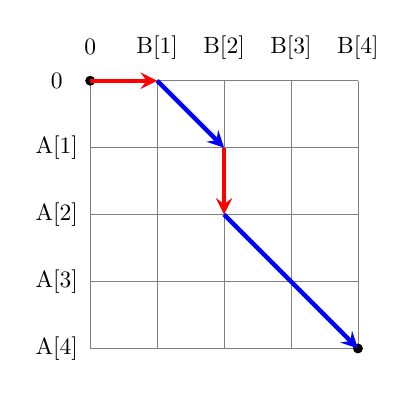
\begin{tikzpicture}[
    scale=0.85, transform shape,
    grid/.style={very thin,gray},
    path/.style={ultra thick,red,->,>=stealth},
    match/.style={ultra thick,blue,->,>=stealth}
]

% Grid lines
\draw[grid] (0,0) grid (4,4);

% Labels
\node at (-0.5,4) {0};
\node at (-0.5,3) {A[1]};
\node at (-0.5,2) {A[2]};
\node at (-0.5,1) {A[3]};
\node at (-0.5,0) {A[4]};

\node at (0,4.5) {0};
\node at (1,4.5) {B[1]};
\node at (2,4.5) {B[2]};
\node at (3,4.5) {B[3]};
\node at (4,4.5) {B[4]};

% Nodes
\node[circle,fill=black,inner sep=1.5pt] (start) at (0,4) {};
\node[circle,fill=black,inner sep=1.5pt] (end) at (4,0) {};

% Path moves
\draw[path] (0,4) -- (1,4); % Insert B[1]
\draw[match] (1,4) -- (2,3); % Match diagonal
\draw[path] (2,3) -- (2,2); % Delete A[2]
\draw[match] (2,2) -- (4,0); % Complete path with matches

\end{tikzpicture}
\caption{Myers Diff Edit Graph Grid}
\end{figure}

\section{AST Diff Syntax Verification Pipeline}

When the LLM outputs a diff patch, applying it blindly can corrupt active workspace files. Production engines execute an **AST Verification Pipeline** on code buffers in memory before saving them to disk.


\begin{center}
\noindent\rule{0.6\textwidth}{0.4pt} \\
\vspace{0.3em}
\textit{[Code implementation is available in the companion coding handbook: \texttt{coding-handbook/ch11\_ai\_ides/}]} \\
\noindent\rule{0.6\textwidth}{0.4pt}
\end{center}


If the AST validation returns `False`, the write is blocked, and the compiler diagnostic is fed back to the LLM to trigger a repair cycle.

\subsection{Python Implementation of Myers Diff}
This algorithm uses a list $V$ where index $k = x - y$ tracks the furthest reaching path on diagonal $k$.


\begin{center}
\noindent\rule{0.6\textwidth}{0.4pt} \\
\vspace{0.3em}
\textit{[Code implementation is available in the companion coding handbook: \texttt{coding-handbook/ch11\_ai\_ides/}]} \\
\noindent\rule{0.6\textwidth}{0.4pt}
\end{center}

